\chapter{Appendix}
\begin{figure}[!ht]
    \centering
    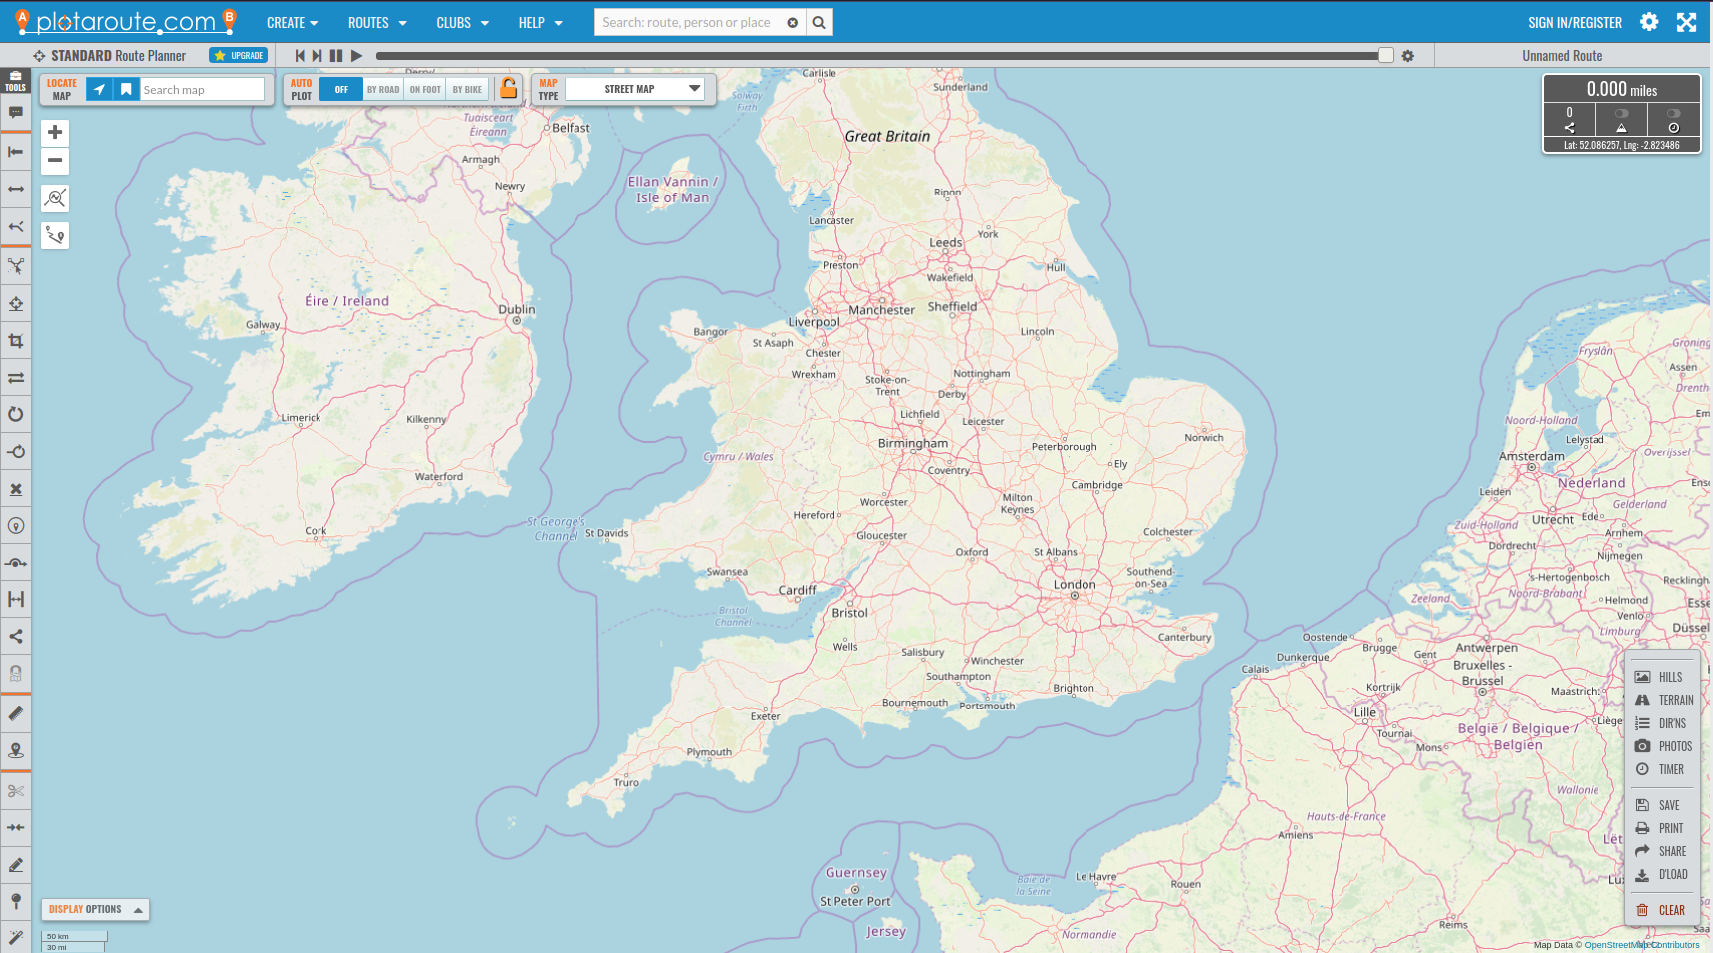
\includegraphics[width=1\linewidth]{figures/plotarouteui.png}
    \caption{Plotaroute.com UI}
    \label{fig:plotarouteui}
\end{figure}

\begin{figure}[!ht]
    \centering
    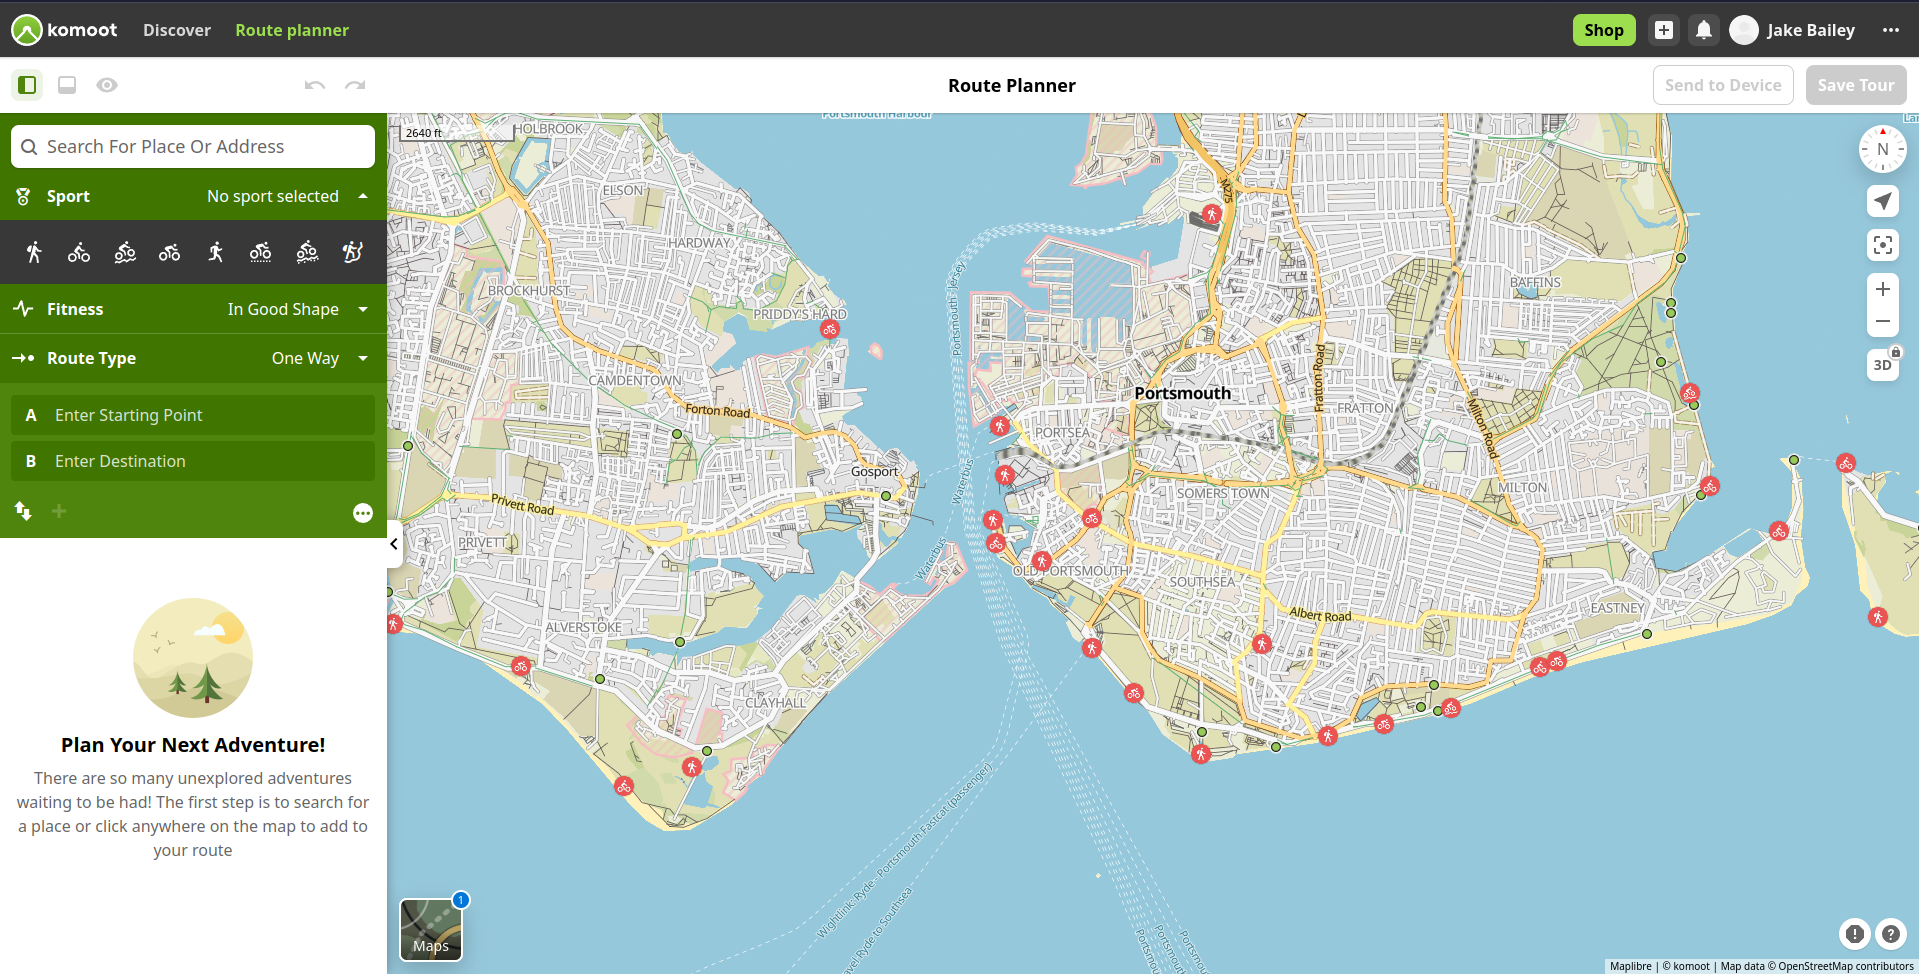
\includegraphics[width=1\linewidth]{figures/komootui.png}
    \caption{Komoot UI}
    \label{fig:komootui}
\end{figure}

\begin{figure}[!ht]
    \centering
    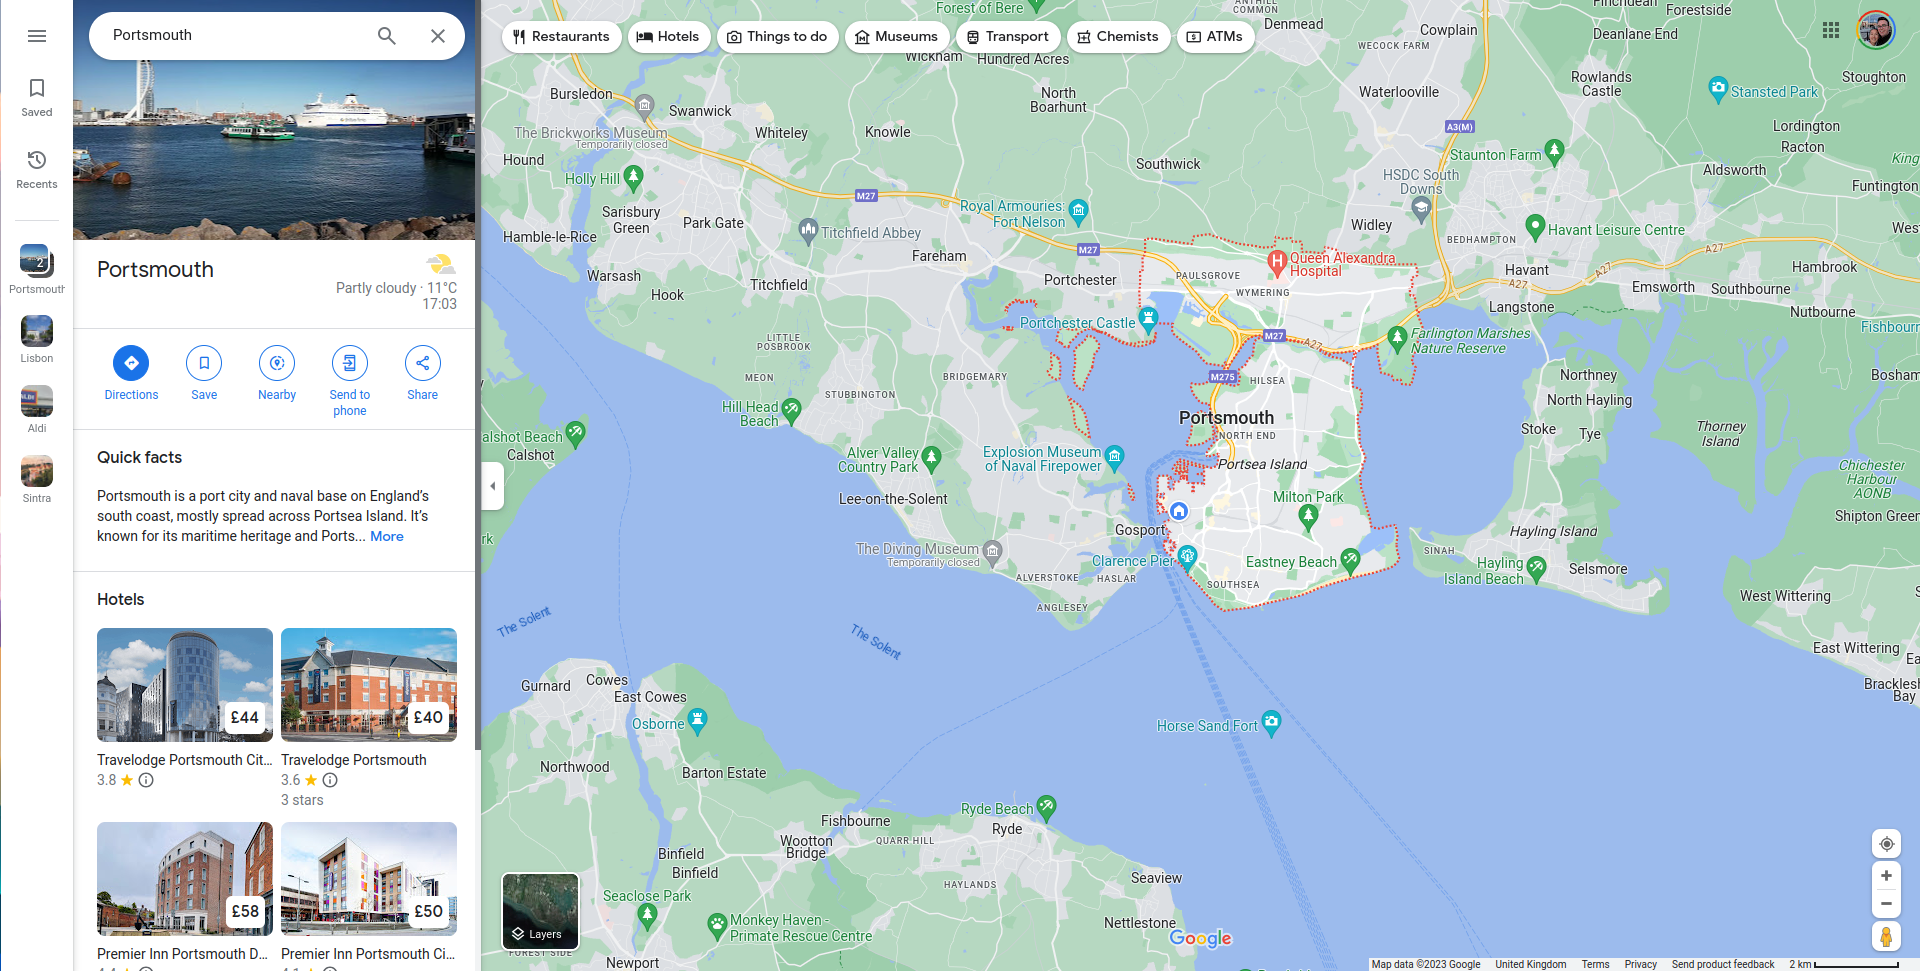
\includegraphics[width=1\linewidth]{figures/gmapsui.png}
    \caption{Google Maps UI}
    \label{fig:gmapsui}
\end{figure}

\clearpage
\section*{Initial User Requirements}
\begin{table}[!h]
\caption{User Story 01}
\label{tab:user-story-01}
\begin{tabular}{ p{8cm} p{1cm}  p{1cm} }
\hline
\multicolumn{3}{p{13cm}}{As a user, I want a page that allows me to configure my starting and destination location to plan a route.}\\ 
\hline
Acceptance Criteria / System Requirements & Priority & ID\\
\hline
The system must provide a route configuration page. & Must & SR1\\
The route configuration page must provide a starting location input field. & Must & SR2\\
The route configuration page must provide a destination location input field. & Must & SR3\\ 
The route configuration page should suggest locations based on the user input fields. & Should & SR4\\ 
The route configuration page must find the location position based on the user input. & Must & SR5\\ 
The route configuration page must verify both locations are correct before the user can continue. & Must & SR6\\ 
The route configuration page must provide a ‘Plan’ button to initiate the route planning algorithm. & Must & SR7\\ 
\hline
\end{tabular}
\end{table}

\begin{table}[!htb]
\caption{User Story 02}
\label{tab:user-story-02}
\begin{tabular}{ p{8cm} p{1cm}  p{1cm} }
\hline
\multicolumn{3}{p{13cm}}{As a user, I want to change preferences to allow me to customise the route further, including avoiding certain road types and road altitudes.}\\ 
\hline
Acceptance Criteria / System Requirements & Priority & ID\\
\hline
The system must provide an overlay window to allow the user to update routing preferences. & Must & SR8 \\
The update preferences overlay must provide an 'avoid' user input field. & Must & SR9\\
The update preferences overlay must provide a 'via' user input field. & Should & SR10\\ 
The update preferences overlay must provide a 'leave time' user input field. & Should & SR11\\ 
The update preferences overlay must provide a 'arrive time' user input field. & Should & SR12\\ 
The update preferences overlay must provide a 'round trip' user input field. & Could & SR13\\ 
\hline
\end{tabular}
\end{table}

\begin{table}[!htb]
\caption{User Story 03}
\label{tab:user-story-03}
\begin{tabular}{ p{8cm} p{1cm}  p{1cm} }
\hline
\multicolumn{3}{p{13cm}}{As a user, I want to be able to export the planned route for use on my mobile phone or GPS device.}\\ 
\hline
Acceptance Criteria / System Requirements & Priority & ID\\
\hline
The system must provide an option to export the planned route. & Must & SR14 \\
The system must provide an export feature to export the route to the 'GPX' file format. & Must & SR15\\
The system must provide an export feature to export the route to the 'GeoJSON' file format. & Should & SR16\\ 
The system must provide an export feature to export the route direct to Strava. & Could & SR17\\ 
\hline
\end{tabular}
\end{table}

\begin{table}[!htb]
\caption{User Story 04}
\label{tab:user-story-04}
\begin{tabular}{ p{8cm} p{1cm}  p{1cm} }
\hline
\multicolumn{3}{p{13cm}}{As a user, I want to share my route with other people.}\\ 
\hline
Acceptance Criteria / System Requirements & Priority & ID\\
\hline
The system must provide a share functionality overlay. & Should & SR18 \\
The share overlay must provide the user with the option to share direct over email. & Should & SR19\\
The share overlay must provide the user with the option to share direct over Google Drive. & Could & SR20\\ 
The share overlay must provide the user with the option to share direct over OneDrive. & Could & SR21\\ 
The share overlay must provide the user with the option to share direct over Dropbox. & Could & SR22\\ 
\hline
\end{tabular}
\end{table}

\begin{table}[!htb]
\caption{User Story 05}
\label{tab:user-story-05}
\begin{tabular}{ p{8cm} p{1cm}  p{1cm} }
\hline
\multicolumn{3}{p{13cm}}{As a user, I want to be provided with route suggestions based on predicted weather conditions over the week.}\\ 
\hline
Acceptance Criteria / System Requirements & Priority & ID\\
\hline
The system must provide the user with a weather condition overlay. & Must & SR23 \\
The weather condition overlay must provide the user with the weather for the current day. & Must & SR24\\
The weather condition overlay must provide the user with the weather for the next week. & Should & SR25\\
The weather condition overlay must provide the user with the option to enable weather conditions in the route planning algorithm. & Could & SR26\\ 
The weather condition overlay must provide the user with suggestions on the best days to cycle. & Could & SR27\\ 
\hline
\end{tabular}
\end{table}

\begin{table}[!htb]
\caption{User Story 06}
\label{tab:user-story-06}
\begin{tabular}{ p{8cm} p{1cm}  p{1cm} }
\hline
\multicolumn{3}{p{13cm}}{As a user, I want to view the route in detail and get information about parts of the route.}\\ 
\hline
Acceptance Criteria / System Requirements & Priority & ID\\
\hline
The system must provide the user with an interactive map to display the planned route. & Must & SR28 \\
The interactive map must allow the user to zoom into parts of the planned route. & Must & SR29\\
The interactive map must allow the user to select parts of the route and receive detailed information about that subsection of the route. & Should & SR30\\
The interactive map must allow the user to select and drag the planned route to modify its path. & Should & SR31\\ 
The system must display an altitude graph for the planned route beneath the interactive map. & Should & SR32\\ 
\hline
\end{tabular}
\end{table}

\begin{table}[!htb]
\caption{User Story 07}
\label{tab:user-story-07}
\begin{tabular}{ p{8cm} p{1cm}  p{1cm} }
\hline
\multicolumn{3}{p{13cm}}{As a user, I want to input hazards from routes I have cycled so the next route planned would attempt to avoid that area.}\\ 
\hline
Acceptance Criteria / System Requirements & Priority & ID\\
\hline
The system must provide a user input modal to input Hazard Data. & Must & SR33 \\
The user input modal must provide a Type drop-down menu based on the OSM Hazard Types. & Must & SR34\\
The user input modal must provide a date entry point to specify the date the hazard was seen. & Should & SR35\\
The user input modal must provide a submit button to add the hazard to the hazard index. & Must & SR35\\ 
\hline
\end{tabular}
\end{table}